% This is a sample LaTeX input file.  (Version of 9 April 1986)
%
% A '%' character causes TeX to ignore all remaining text on the line,
% and is used for comments like this one.

% Rob Phillips lifted from /usr/local/lib/tex/inputs/sample.tex
% to use as template.

\documentclass[12pt]{article}    % Specifies the document style.

 \usepackage[pdftex]{graphicx}
\input{epsf}

\usepackage{fancyhdr}
\usepackage{extramarks}
\usepackage{amsmath}
\usepackage{amsthm}
\usepackage{amsfonts}
\usepackage{tikz}
\usepackage{tcolorbox}
\tcbuselibrary{breakable}
\usepackage{mathtools}
\usepackage{color,soul}
\usepackage{mdframed}
\usepackage{graphicx}
\usetikzlibrary{automata,positioning}
\usepackage{environ}
\usepackage{hyperref}
\usepackage{xcolor}

\newcommand{\ee}{\varepsilon}
\newcommand{\DD}{\Delta}
\newcommand{\dd}[1]{{\partial \over \partial {#1}}}
\newcommand{\ddd}[1]{{\partial^2 \over \partial {#1} ^2}}

                           % The preamble begins here.
\begin{document}           % End of preamble and beginning of text.
\relax


\begin{center}
{\bf\Large Bi/Ge105: Evolution}\\
{\bf\Large Homework 3}\\
{\bf\Large Due Date: Thursday, March 01, 2018}\\
\end{center}

\section{Problem 1: Genetic Drift as a Force of Evolution}
\subsection{Simulating the  processes of evolution}

In class we learned about the mathematical formalism behind population
genetics, one of the centerpieces of evolutionary theory. The ideas described in
class will provide a quantitative backdrop for understanding the different
evolutionary forces that shape life on our planet. It is both profound and
amusing how much we can learn about evolution by thinking about coin flips and
similar games of chance. Indeed, the broad reach of the mathematics of coin
flips is an example of what former Caltech undergrad and now Harvard professor
\href{http://www.people.fas.harvard.edu/~blitz/Site/Home.html}{Joe Blitzstein}
likes to say: ``The nouns change, but the verbs remain the same.'' \\

In this  problem we want you to explore different evolutionary forces by means
of simulations. You will use what you learned in the \textit{stochastic
simulation} tutorial to explore the interplay of different evolutionary forces
such as genetic drift and mutation. By using simulations we will sidestep more
advanced mathematics of stochastic differential equations  needed to study these
concepts analytically while still getting clear insights into how these forces
may affect the course of evolution.

\subsection{The Buri genetic drift experiment}

In 1956 Peter Buri, a student of
\href{https://en.wikipedia.org/wiki/Sewall_Wright}{Sewall Wright} published the
now classic paper ``\textit{Gene Frequency in Small Populations of Mutant
Drosophila}'' in which he experimentally demonstrated the concept of genetic
drift.  The idea for this beautiful experiment is depicted in
Fig. \ref{figBuriSchematic}. Briefly, Buri began with eight female and eight male
flies, all heterozygotes of the \textit{bw} locus. This means that all of the
flies had 1 copy of the gene associated with white eyes, and one copy of the
gene associated with  red eyes. The phenotype that this combination of alleles
gives is flies with orange eyes. He then allowed the flies to reproduce, and
after removing the adults, he randomly chose 8 males and females from the next
generation of offspring without looking at the eye color. These new 8 males and
8 females were transferred to a new flask and the procedure was repeated for 19
generations.

\begin{figure}[h!]
\centering{
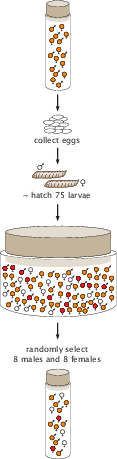
\includegraphics[scale=0.8]{BuriSchematic}\label{figBuriSchematic}
\caption{{\bf Buri's experimental setup.} At time $t=0$ eight
heterozygote females and eight heterozygote males were allowed to reproduce.
From their offspring, eight males and eight females were chosen at random and
transferred into a new flask.}}
\end{figure}

\vspace{5mm}
\textbf{Question 1a:} Work out what is the expected genotype frequency of
red-eyed flies, white-eyed flies and orange-eyed flies after the first
generation. (Hint: Recall that each allele is drawn from the parent's pool
\textbf{at random with replacement}. This means that to compute the frequency of
red-eyed flies you should calculate $f_{rr} = P(\text{red allele first draw})
\cdot P(\text{red allele second draw})$.
\vspace{5mm}

Since the offspring that made it to the next generation were chosen at random,
Buri knew that the outcome would be different if he repeated an identical
experiment in different vials. As a result, for statistical power he simultaneously tracked
107 flasks as
shown in Fig. \ref{figBuriSchematic}. Each generation, he counted the number of red-eyed, white-eyed and orange-eyed flies he had randomly chosen.
Fig. \ref{figBuriGenerations} shows the outcomes for these different vials after 19
generations. Because the flies are allegedly mating at random, with each
generation there is an accumulation of fluctuations. As a result, after 19
generations, many vials contained only white-eyed or red-eyed flies, though
some vials still contained a mixture of eye colors.

\begin{figure}[h!]
\centering{
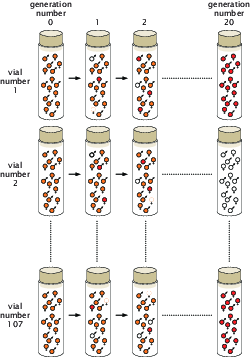
\includegraphics[scale=0.7]{BuriGenerations}
\caption{{\bf Multiple replicates of the Buri experiment.}  Buri repeated
his experiment in 107 separate vials, with the evolutionary trajectory
different each time as a result of genetic drift.  Note that in the long time limit,
many of the vials have gone to fixation with all flies having either white or red eyes.
}
\label{figBuriGenerations}}
\end{figure}

Having quantified the number of red-eyed, white-eyed and orange-eyed flies Buri
was able to quantify the frequency of alleles in the population. Since none of
the alleles were dominant, he could infer the genotype  by
looking at the phenotype of the flies.

\vspace{5mm}
\textbf{Question 1b:} Write down the formula for the genotype frequencies in
terms of the eye color count.  Use the notation $N_{red}$ for the number of
red-eyed flies in a given vial, $N_{white}$ for the number of white-eyed flies
in that same vial and finally, $N_{orange}$ for the number of orange-eyed flies
in that same vial.  Your task is to figure out the frequency of red ($f_r$) and
white ($f_w$) alleles in a given vial given the counts of the number of red-,
white- and orange-eyed flies.
\vspace{5mm}


Fig. \ref{figBuriExperiment} summarizes the
results of the experiment. By tracking alleles over time with these 107
populations exposed to the same conditions, Buri was able to observe evolution
driven entirely by genetic drift! He saw how in some of the populations one of
the alleles went extinct, arising from nothing more than the fluctuations inherent in small
populations.

\begin{figure}[h!]
\centering{
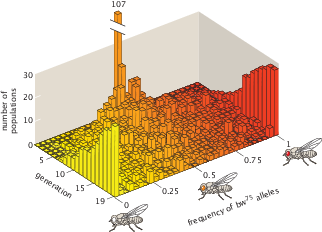
\includegraphics[scale=0.85]{BuriExperiment}
\caption{{\bf Results of the Buri experiment.} By tracking the phenotypes of the
flies, Buri was able to infer the allele frequencies for each population. The
allele frequencies change as a result of genetic drift and after 19 generations,
many of the vials contain flies all with the same eye color, implying fixation
of alleles and evolution due to genetic drift.}
\label{figBuriExperiment}}
\end{figure}

It is now time for us to use our computational prowess to simulate and explore
the Buri experiment.

\subsection{Reproducing the Buri experiment \textit{in-silico}}
Your first task will be to reproduce Fig. \ref{figBuriExperiment} by means of
stochastic simulations. The key elements of the code you need to
do this analysis you already worked out in the stochastic
simulation tutorial.

\vspace{5mm}
\textbf{Question 1c:} Perform stochastic simulations of genetic drift for 107
populations over 19 generations using the same population size as Buri, i.e.
16 flies total (32 alleles). Plot histograms of the allele frequency for
generation numbers 0, 1, 10, and 19.
\vspace{5mm}

\subsection{The effect of the population size}
 Using these exact same tools we will now explore the effect
 of the population size.

\vspace{5mm}
\textbf{Question 1d:} Repeat the stochastic simulations for 107 populations
during 1000 generations using the same population size as Buri. Quantify the
time it takes for each of these populations to have one of the alleles fixed,
i.e. find the time point for each population at which the allele frequency
becomes either zero or one, and save the generation number at which this
happened. Now repeat the simulation for varying population size ($ N = $ 4, 8,
16, 32, and 64). Plot the mean time to fixation as a function of the population
size and comment on how this average time to fixation scales as the population
size changes. What do these results mean for the role genetic drift
plays in different populations? (Hint: to find which generation one of the
alleles was fixed in the population, the function \texttt{numpy.where} might
become handy. Basically you just need to find a way for Python to tell you at
which entry of the array the frequency became \texttt{f == 1} \textbf{or}
\texttt{f == 0}. You might also want to check the \texttt{numpy.logical\_or}
function that allows you to perform boolean \texttt{or} operations over numpy
arrays.)
\vspace{5mm}

\subsection{The effect of mutations}

Let's now explore the effect of another evolutionary force -- mutation. In
our toy model, rather than thinking about tracking the complexity of single base
pair mutations, we will think of a ``reaction'' of the following form
\begin{equation}
A \xrightleftharpoons[\mu_2]{\mu_1} a
\end{equation}
where $A$ and $a$ are the two versions of the allele (for example red and
white), and $\mu_1$ and $\mu_2$ are the mutation rates that take you from one
allele to the other. To simplify things even further we will assume $\mu_1 =
\mu_2 \equiv \mu$.

\vspace{5mm}
\textbf{Question 1e:} Implement a stochastic simulation to include the effect of
mutation for a single population and plot the allele frequency over time.
Comment on the differences with respect to the case without mutation. (Hint: The
mating still happens at random in this scenario, but now each allele after being
selected for the next generation must flip a second coin to decide if it
remains as the same allele, or it mutates into the other allele). Use the value
$\mu \approx 0.001$ for your simulations.
\vspace{5mm}

\vspace{5mm}
\textbf{Question 1f:} Extend the algorithm you just wrote and simulate 100
populations. Plot 10 of these trajectories, as well as histograms of allele
frequency at representative time points such as $t = 0, 5, 10, 50, 100, 500$
generations. Compare this to the null model where the mutation rate is equal
to zero and comment on the differences if any between the distributions over
time.
\vspace{5mm}

\vspace{5mm}
\textbf{Question 1g:} You will now explore the effect of the magnitude of the
mutation rate. Run the simulation for 100 generations for $\mu =$0,  0.001,
0.01, 0.1 and plot the histogram of allele frequencies of the final time point
for each of these mutation rates. Comment on how the distribution changes as the
mutation rate increases.
\vspace{5mm}

%%%%%%%%%%%%%%%%%%%%%%%%%%%%
%%%%%%%%%%%%%%%%%%%%%%%%%%%%
%%%%%%%%%%%%%%%%%%%%%%%%%%%%

\clearpage

\section{Problem 2: Symbiosis as a driving force of evolution.}

\noindent

\textbf{Question 2a:} In class we discussed the arms race between the poisonous
rough skinned newt and garter snakes and the observed increased resistance to
the toxin by the predator. How does the newt (or another toxin producing
organism) avoid poisoning itself? Find an example in the literature, describe
the mechanism in 1-2 paragraphs and cite the source.

\vspace{5mm}
\textbf{Question 2b:} How would you go about characterizing the taxonomy a new
organism whose genome was 1/3 eucaryotic, 1/3 archaeal, and 1/3 bacterial?

% \section{Problem 2: Experimental evolution in the era of genome sequencing}
%
% Within the past two decades, sequencing an organisms' entire genome has become a
% nearly trivial procedure. This affords us the ability to observe evolution at
% the genetic level in real time. This has opened up an exciting new field in
% which the technology of next-generation sequencing is combined with the
% experimental advantage of microbial systems making it possible to test
% quantitative evolutionary theories.
%
% A particularly interesting long-term experiment involves Professor
% Richard Lenski at Michigan
% State University. On February 24, 1988,
% \href{http://myxo.css.msu.edu/index.html}{Lenski} began growing twelve
% \textit{E. coli} cultures in parallel, similar to Buri's experiment from problem
% 1 but in a haploid world with organisms with generation times of around one
% hour. Twenty-nine years and almost 70,000 generations later this experiment has watched more generations of evolution than any other experiment ever done.
%
%
% These bacterial cultures have been adapting to a very simple environment with a fixed
% media composition. The advantage of working with these microbes is that every
% certain number of generations a sample can be frozen and brought back to life at
% will. In this sense, Lenski's $-80^\circ$C freezers act as an evolutionary
% time-machine, allowing him to recover organisms from the ``fossil record''!
%
% One surprising outcome of this experiment is the appearance of a bacterial
% strain capable of metabolizing a new carbon source. For historical reasons (most
% likely to avoid phage infection) the cultures have always been grown in the
% presence of \href{https://en.wikipedia.org/wiki/Citric_acid}{citrate}. Back in
% the day, before the sequencing revolution, one of the ways to identify bacterial
% species was by their metabolic repertoire. Scientists would classify a
% bacterium as \textit{E. coli} for example based on its ability to ferment
% arabinose, lactose, mannitol, and the \textbf{lack of ability} to ferment
% citrate, among other things
% (look at
% \href{http://www.microbiologyinfo.com/biochemical-test-and-identification-of-e-coli/}{this
% site} for a complete list of the features). So in principle if you were to
% collect a sample from the soil that was able to ferment citrate you would
% immediately conclude it was not a wild-type \textit{E. coli} strain.
%
% In fact,  \textit{E. coli} does contain the machinery to ferment citrate
% encoded in its genome, but this set of genes is only expressed under anaerobic
% conditions. Lenski found that in one of his 12 replicate populations bacteria
% were able to metabolize citrate under aerobic conditions. This means that once
% the glucose that is found initially in the media runs out, this mutant strain
% can still grow further before the culture is diluted the next morning, giving it
% a clear fitness advantage over its competitors!
%
% In this problem we will work out a very simple equation to analyze how long
% it would take for this mutant to overtake the culture.
%
% \subsection{Toy model for two competing bacteria strains}
%
% Consider the case in which two alleles, $A_1$ and $A_2$, are present in a
% population with initial frequency $p$ and $q = 1 - p$, respectively. For example, these
% alleles could be those associated with the ability to metabolize citrate or not.
%  Let us assume that cells harboring allele $A_1$ have a growth rate
% $m_1$ and those harboring $A_2$ have a growth rate $m_2$.  When thinking
% about
% microbial organisms the growth rate is often taken as a metric for fitness and it's
% given the name of
% \href{http://mathworld.wolfram.com/MalthusianParameter.html}{Malthusian
% parameter}. For natural selection to act on organisms there must be a difference
% in fitness, otherwise if all organisms had the same fitness, no Darwinian
% evolution would occur.
% %In that sense fitness plays a similar role in
% %evolution to what energy does in thermodynamics in which only differences in
% %energy are relevant for reactions to happen.
%
% Let us further assume that $A_1$ represents the allele that allows bacteria to
% metabolize citrate, and as a consequence $m_1 > m_2$. In particular we will say
% that $m_2 = m_1 (1 - s)$, where $s$ is a small parameter $s \ll 1$. If $N_1$ represents the number
% of cells with allele $A_1$, and $N_2$ the number of cells with allele $A_2$, the
% equation that describes the growth curve is given by
% \begin{equation}
% 	\frac{dN_i}{dt} = m_i N_i,
% \end{equation}
% for $i \in \{1, 2\}$. The solution to this differential equation results in
% an exponential growth profile, namely,
% \begin{equation}\label{eq_n_t}
% 	N_i(t) = N_i (0) e^{m_i t},
% \end{equation}
% where $N_i(0)$ is the initial number of cells with allele $A_i$.
%
% \vspace{5mm}
% \textbf{Question 2a:} Write an expression for $N_{tot}(t)$ the total number of
% cells as a function of time. (Hint: Remember we have two competing cell types
% and we are assuming they don't interfere with each other).
% \vspace{5mm}
%
% Having this expression for $N_{tot}(t)$ is interesting. But what we really care
% about is the frequency of alleles in the population given that one of the
% alleles has a fitness advantage over the other. This means that the quantity we
% care about is the \textbf{normalized frequency} $p(t)$.
%
% \vspace{5mm}
% \textbf{Question 2b:} Write an expression for $p(t)$, the frequency of the
% mutant allele $A_1$ and another expression for $q(t)$, the frequency of the
% wild-type allele $A_2$ as a function of time. This should be a function of the
% initial cell count $N_1(0)$ and $N_2(0)$, as well as the selection coefficient
% $s$. Simplify this result to an expression of the form
% \begin{equation}
%   p(t) = \frac{1}{1 + f(t)}.
% \end{equation}
% \vspace{5mm}
%
% Hopefully you ended up with a nice, compact expression that looks like a
% logistic function. Let's now explore the consequences of this expression.
%
% \vspace{5mm}
% \textbf{Question 2c:} Let $p(0)$, the initial frequency of $A_1$, be $10^{-9}$.
% Assume the doubling time of the mutant is 1 hour, then plot $p(t)$ and $q(t)$
% for different selection coefficients, $s = 10^{-4}, 10^{-3}, 10^{-2}$. Label the
% $x$ axis as years rather than hours to have a better sense of how long it would
% take for the mutants to overtake the population. (Hint: It might be useful to
% plot this both on a linear scale and on a log scale for the $x$ axis.)
% \vspace{5mm}
%
% \clearpage
% \noindent {\bf X. Diffusion of alleles over frequency space}\\
%
% \noindent   In this problem we will work out the details of the beautiful
% diffusion theory. As experimental techniques such as robotics for culture
% handling and sequencing open the doors to ask new questions about evolution, now
% more than ever is important to contextualize these results under a unifying
% theoretical framework that explains the structure of the data. We hope that
% going through this derivation will inspire you to think about how the
% interaction between theory and experiment can give us new insights into how
% “endless forms, most beautiful and most wonderful have been, and are being,
% evolved.”
%
% \subsubsection*{Deriving the Fokker-Planck equation for allele diffusion.}
%
% As we did in class, we derive the diffusion equation for a one-loci two-allele
% system following a similar path as Einstein did for the diffusion of particles
% in space. We begin by writing the “continuous master equation” of the form\\
% \begin{equation} \label{eq_master_eq}
%     P(f, t+\DD t \mid f_o, t_o) = \int d\ee
%   P(f - \ee, t \mid f_o, t_o)
%   \phi (f - \ee, \ee; t, \DD t).
% \end{equation}
% The left hand side of the equation is read as "probability of having frequency
% $f$ at time $t + \DD t$ given that we started a frequency $f_o$ at time
% $t_o$". For this case we are being very explicit that the initial condition
% $f_o$ is \textbf{fixed}. This assumption can be relaxed when asking a different
% type of questions. The right hand side of the equation tells us to sum
% (integrate for continuous $f$) over all possible trajectories from
% $f - \ee$ to $f$, where $\phi (f - \ee, \ee; t, \DD
% t)$ dictates the likelihood of making a jump of size $\ee$ when standing
% at position $f - \ee$ at time $t$ during a time interval $\DD t$.
%
% For this derivation we will assume that the process is time homogeneous. What
% that means is that the transition from one point to the next doesn't depend on
% the time. Furthermore we will assume that our transition probability $\phi$ only
% considers time steps fo size $\DD t$. This allow us to simply write
% \begin{equation}
%   \phi (f - \ee, \ee; t, \DD t) =
%   \phi (f - \ee, \ee).
% \end{equation}
%
% To simplify our notation unless specified otherwise we will assume that the
% inital frequency $f_o$ at time $t_o$ is fixed so that we can write
% \begin{equation}
%   P(f, t \mid f_o, t_o) = P(f, t).
% \end{equation}
%
% \noindent
% (a) Perform a Taylor expansion around $f$ up to second order of the integrand
% in Eq. \ref{eq_master_eq}
% \begin{equation}
%   \color{blue}
%   P(f - \ee, t) \phi(f - \ee, \ee) \approx
%   P(f, t) -
%   \ee {\partial \over \partial f}\left[ P(f, t) \phi(f, \ee) \right] +
%   {\ee^2 \over 2!} {\partial^2 \over \partial f^2}
%   \left[ P(f, t) \phi(f, \ee) \right].
% \end{equation}
%
% \noindent
% (b) If we now assume that the order of summation, integration and
% differentiation can be freely interchanged under some minor conditions, rewrite
% Eq. \ref{eq_master_eq} using your Taylor expansion and noting that
% \begin{equation}\label{eq_norm_jump}
%   \int \phi(f, \ee) d\ee = 1,
% \end{equation}
% i.e. the probability of making a jump of any size is equal to 1.
% \begin{equation}
%   \color{blue}\scriptstyle
%   P(f, t + \DD t) \approx P(f, t) \int d\ee \phi(f, \ee) -
%   \dd{f}\left[ P(f, t) \int d\ee \cdot \ee \cdot \phi(f, \ee) \right] +
%   {1 \over 2} \ddd{f}
%   \left[ P(f, t) \int d\ee \cdot \ee^2 \cdot \phi(f, \ee) \right].
% \end{equation}
% \textcolor{blue}{
% Using Eq. \ref{eq_norm_jump} we have
% }
% \begin{equation}
%   \color{blue}\scriptstyle
%   P(f, t + \DD t) \approx P(f, t) -
%   \dd{f}\left[ P(f, t) \int d\ee \cdot \ee \cdot \phi(f, \ee) \right] +
%   {1 \over 2} \ddd{f}
%   \left[ P(f, t) \int d\ee \cdot \ee^2 \cdot \phi(f, \ee) \right].
% \end{equation}
%
% \noindent
% (c) Rearrange your answer from part (b) by sending terms that do not involve
% derivatives to the left hand side of the equation and dividing both sides by
% $\DD t$. Then take the limit when $\DD t \rightarrow 0$ to obtain a PDE on $t$.
% \begin{equation}
%   \color{blue}\scriptstyle
%   \lim_{\DD t \rightarrow 0} {P(f, t + \DD t) - P(f, t) \over \DD t} \approx
%   \lim_{\DD t \rightarrow 0} -
%   \dd{f}\left[ P(f, t) \int d\ee \cdot \ee \cdot \phi(f, \ee) \right] +
%   {1 \over 2} \ddd{f}
%   \left[ P(f, t) \int d\ee \cdot \ee^2 \cdot \phi(f, \ee) \right].
% \end{equation}
% \textcolor{blue}{
% Taking the limit gives
% }
% \begin{equation}\label{eq_master_expansion}
%   \color{blue}\scriptstyle
%   \dd{t}P(f, t) \approx
%   \lim_{\DD t \rightarrow 0} -
%   \dd{f}\left[ P(f, t) {1 \over \DD t}
%   \int d\ee \cdot \ee \cdot \phi(f, \ee) \right] +
%   {1 \over 2} \ddd{f}
%   \left[ P(f, t) {1 \over \DD t}
%   \int d\ee \cdot \ee^2 \cdot \phi(f, \ee) \right].
% \end{equation}
%
% \noindent
% (d) To complete the derivation of the Fokker-Planck equation (or the Kolmogorov
% forward equation if you are a mathematician) use the following definitions
% \begin{align}
%   M(f) &\equiv
%   \lim_{\DD t \rightarrow 0} {1 \over \DD t}
%   \left[ \int d\ee \cdot \ee \cdot \phi(f, \ee) \right],\\
%   V(f) &\equiv
%   \lim_{\DD t \rightarrow 0} {1 \over \DD t}
%   \left[ \int d\ee \cdot \ee^2 \cdot \phi(f, \ee) \right].
% \end{align}
% And rewrite Eq. \ref{eq_master_expansion} using these definitions.
% \begin{equation}
%   \color{blue}
%   \dd{t}P(f, t) = - \dd{f}\left[ P(f, t) M(f) \right] +
%   {1 \over 2} \ddd{f}\left[ P(f, t) V(f) \right].
% \end{equation}
%
% \subsubsection*{Computing the steady-state distribution}
%
% In order to compute the steady state distribution of allele frequency for our
% system we will extent the analogy of diffusion of particles in space. You might
% recall from an obscure physics or chemistry class that Fick's laws relate fluxes
% and concentrations. Specifically we have that Fick's first law relates the
% diffusive flux to the concentration. For a 1D system undergoing only diffusion
% the law is stated as
% \begin{equation}\label{eq_fick_first}
%   J = - D \dd{x} c,
% \end{equation}
% where $J \equiv J(x, t)$ is the diffusive flux, $D$ is the diffusion
% coefficient, and $c \equiv c(x, t)$ is the concentration profile as a function
% of the space $x$ and time $t$.
%
% If the system is undergoing not only diffusion but some directional drift, the
% flux of the system then is written as
% \begin{equation}\label{eq_diff_conv}
%   J = - D \dd{x} c + f(x)c(x, t),
% \end{equation}
% where $f(x)$ is the a function that determines the drift for each spatial
% coordinate $x$.
%
% {\bf Note:} This is an unfortunate use of vocabulary. In physics the drift term
% implies \textit{directional} movement, while in population genetics drift refers
% to the \textit{random} sampling of alleles. To distinguish both drifts we will
% always refer to the population genetics drift as {\bf random drift}.
%
% Fick's second law is equivalent to the diffusion equation. It relates the
% diffusive flux to the changes of concentration in time. This law is usually
% written as
% \begin{equation}\label{eq_fick_second}
%   \dd{t} c = \dd{x}J.
% \end{equation}
%
% \noindent
% (e) Substitute Eq. \ref{eq_diff_conv} into Eq. \ref{eq_fick_second} and show
% that this gives back the diffusion-convection equation.
% \begin{equation}
%   \color{blue}
%   \dd{t} c = \dd{x} \left[ -D \dd{x}c + f(x)c(x,t) \right].
% \end{equation}
% \textcolor{blue}{
% This gives
% }
% \begin{equation}
%   \color{blue}
%   \dd{t}c = - D \ddd{x}c + \dd{x}\left[ f(x)c(x, t) \right]
% \end{equation}
%
% As discussed in class, the main difference between the usual spatial diffusion
% and the diffusion of alleles in frequency space is that the diffusion
% coefficient in our case is a function of the frequency. Nevertheless for a 1D
% system it must be true that at steady state the flux $J(x) = 0$. We emphasize
% that this is true only for the 1D case, because there is only one forward and
% one backwards direction so the flow on each direction must be the same. If there
% were three possible directions the steady-state wouldn't necessarily imply no
% flux since there could be a stead movement from state 1 to state 2 to state 3
% and back to state 1 giving a non-zero net flux.
%
% \noindent
% (f) Compute the steady-state distribution for your answer in part (d) by setting
% the time derivative to zero and integrating the terms with respect to $f$. At
% this point you should end up with a first-order linear ODE with an undetermined
% integration constant $C$.
% \begin{equation}
%   \color{blue}
%   0 = - \dd{f}\left[ P(f) M(f) \right] +
%   {1 \over 2} \ddd{f}\left[ P(f) V(f) \right].
% \end{equation}
% \textcolor{blue}{
% Integrating both sides with respect to $f$ gives
% \begin{equation}
%   \color{blue}
%   \int 0 df = - \int df \dd{f}\left[ P(f) M(f) \right] +
%   \int df {1 \over 2} \ddd{f}\left[ P(f) V(f) \right].
% \end{equation}
% Computing these integrals give
% \begin{equation}
% C = - P(f)M(f) + {1 \over 2} \dd{f} \left[ P(f) V(f) \right],
% \end{equation}
% where $C$ is an integration constant.
% }
%
% The difference between Eq. \ref{eq_diff_conv} and your answer for part (f) is
% that the diffusion coefficient should remain inside the derivative with respect
% to the frequency coordinate. We can now use our analogy with spatial diffusion
% to find the value of the integrating constant.
%
% \noindent
% (g) Use the fact that for a 1D system the steady state flux must satisfy $J(x)
% = 0$ to solve for the integration constant $C$.
%
% \textcolor{blue}{
% Since the answer for part (f) is equivalent to Eq. \ref{eq_diff_conv}, the
% integration constant must be zero.
% }
%
% \noindent
% (h) Arrange the equation to obtain a first-order homogeneous ODE .Clue: Define
% the following function $G(f) \equiv P(f)V(f)$.
%
% \textcolor{blue}{
% Using the definition of the function $G(f)$ gives
% \begin{equation}
%   0 = - {G(f) M(f) \over V(f)} + {1 \over 2} \dd{f}G(f).
% \end{equation}
% We can rearrange terms to write it in a standard form as
% \begin{equation}
%   \dd{f}G(f) - 2 G(f)\cdot {M(f) \over V(f)} = 0.
% \end{equation}
% And this is our first-order homogeneous differential equation.
% }
%
% \noindent
% (i) Solve the equation using the method of the integrating factor.
%
% \textcolor{blue}{
% We can multiply both sides of the equation by $\exp \left[
% -2 \int df {M(f) \over V(f)} \right]$, obtaining
% \begin{equation}
%   \dd{f}G(f) \cdot \exp\left[ -2 \int df {M(f) \over V(f)} \right] -
%   2 G(f) {M(f) \over V(f)} \exp\left[ -2 \int df {M(f) \over V(f)} \right] = 0
% \end{equation}
% Notice that this is equivalent to writing
% \begin{equation}
% - \dd{f} \left\{ G(f) \exp \left[ -2 \int df {M(f)\over V(f)} \right] \right\}
% = 0
% \end{equation}
% We can now integrate both sides with respect to $f$ obtaining
% \begin{equation}
%   G(f) \exp\left\{ -2 \int df {M(f) \over V(f)} \right\} = C,
% \end{equation}
% where $C$ is an integration constant. Substituting back $G(f)$ gives
% \begin{equation}
%   P(f)V(f) = C \exp\left\{ 2 \int df {M(f) \over V(f)} \right\}.
% \end{equation}
% Therefore the steady-state distribution of allele frequencies is of the form
% \begin{equation}
%   P(f) = {C \over V(f)} \exp\left\{ 2 \int df {M(f) \over V(f)} \right\}.
% \end{equation}
% }

\end{document}             % End of document.
